\section{Descrizione del Modello YOLOv8 per Object Detection}

YOLO (You Only Look Once) è una delle architetture di deep learning più utilizzate per il rilevamento degli oggetti (object detection) in tempo reale. La versione 8 di YOLO, denominata YOLOv8, rappresenta un ulteriore miglioramento rispetto alle versioni precedenti, combinando un'elevata accuratezza con una velocità di esecuzione che la rende ideale per applicazioni in scenari complessi e dinamici, come il riconoscimento dei rifiuti plastici nei bacini idrici.

\subsection{Panoramica di YOLOv8}

YOLOv8 è progettato per fornire un bilanciamento ottimale tra precisione e velocità. La sua architettura è costruita su principi consolidati delle reti convoluzionali, ma con innovazioni che ne migliorano l'efficienza e la capacità di generalizzazione. In particolare, YOLOv8 sfrutta blocchi convoluzionali più leggeri e tecniche di ottimizzazione avanzate che riducono il tempo di inferenza senza sacrificare l'accuratezza.

\subsection{Architettura di YOLOv8}

L'architettura di YOLOv8 si basa su un approccio end-to-end che suddivide l'immagine in una griglia e applica convoluzioni multiple per predire le bounding box e le classi degli oggetti all'interno di ciascuna cella della griglia. YOLOv8 utilizza tecniche avanzate come la \textit{Path Aggregation Network} (PANet) per migliorare l'integrazione delle informazioni a diversi livelli di profondità della rete, il che è fondamentale per rilevare oggetti di varie dimensioni e scale. Di seguito è riportato un diagramma semplificato dell'architettura:

\begin{figure}[h!]
    \centering
    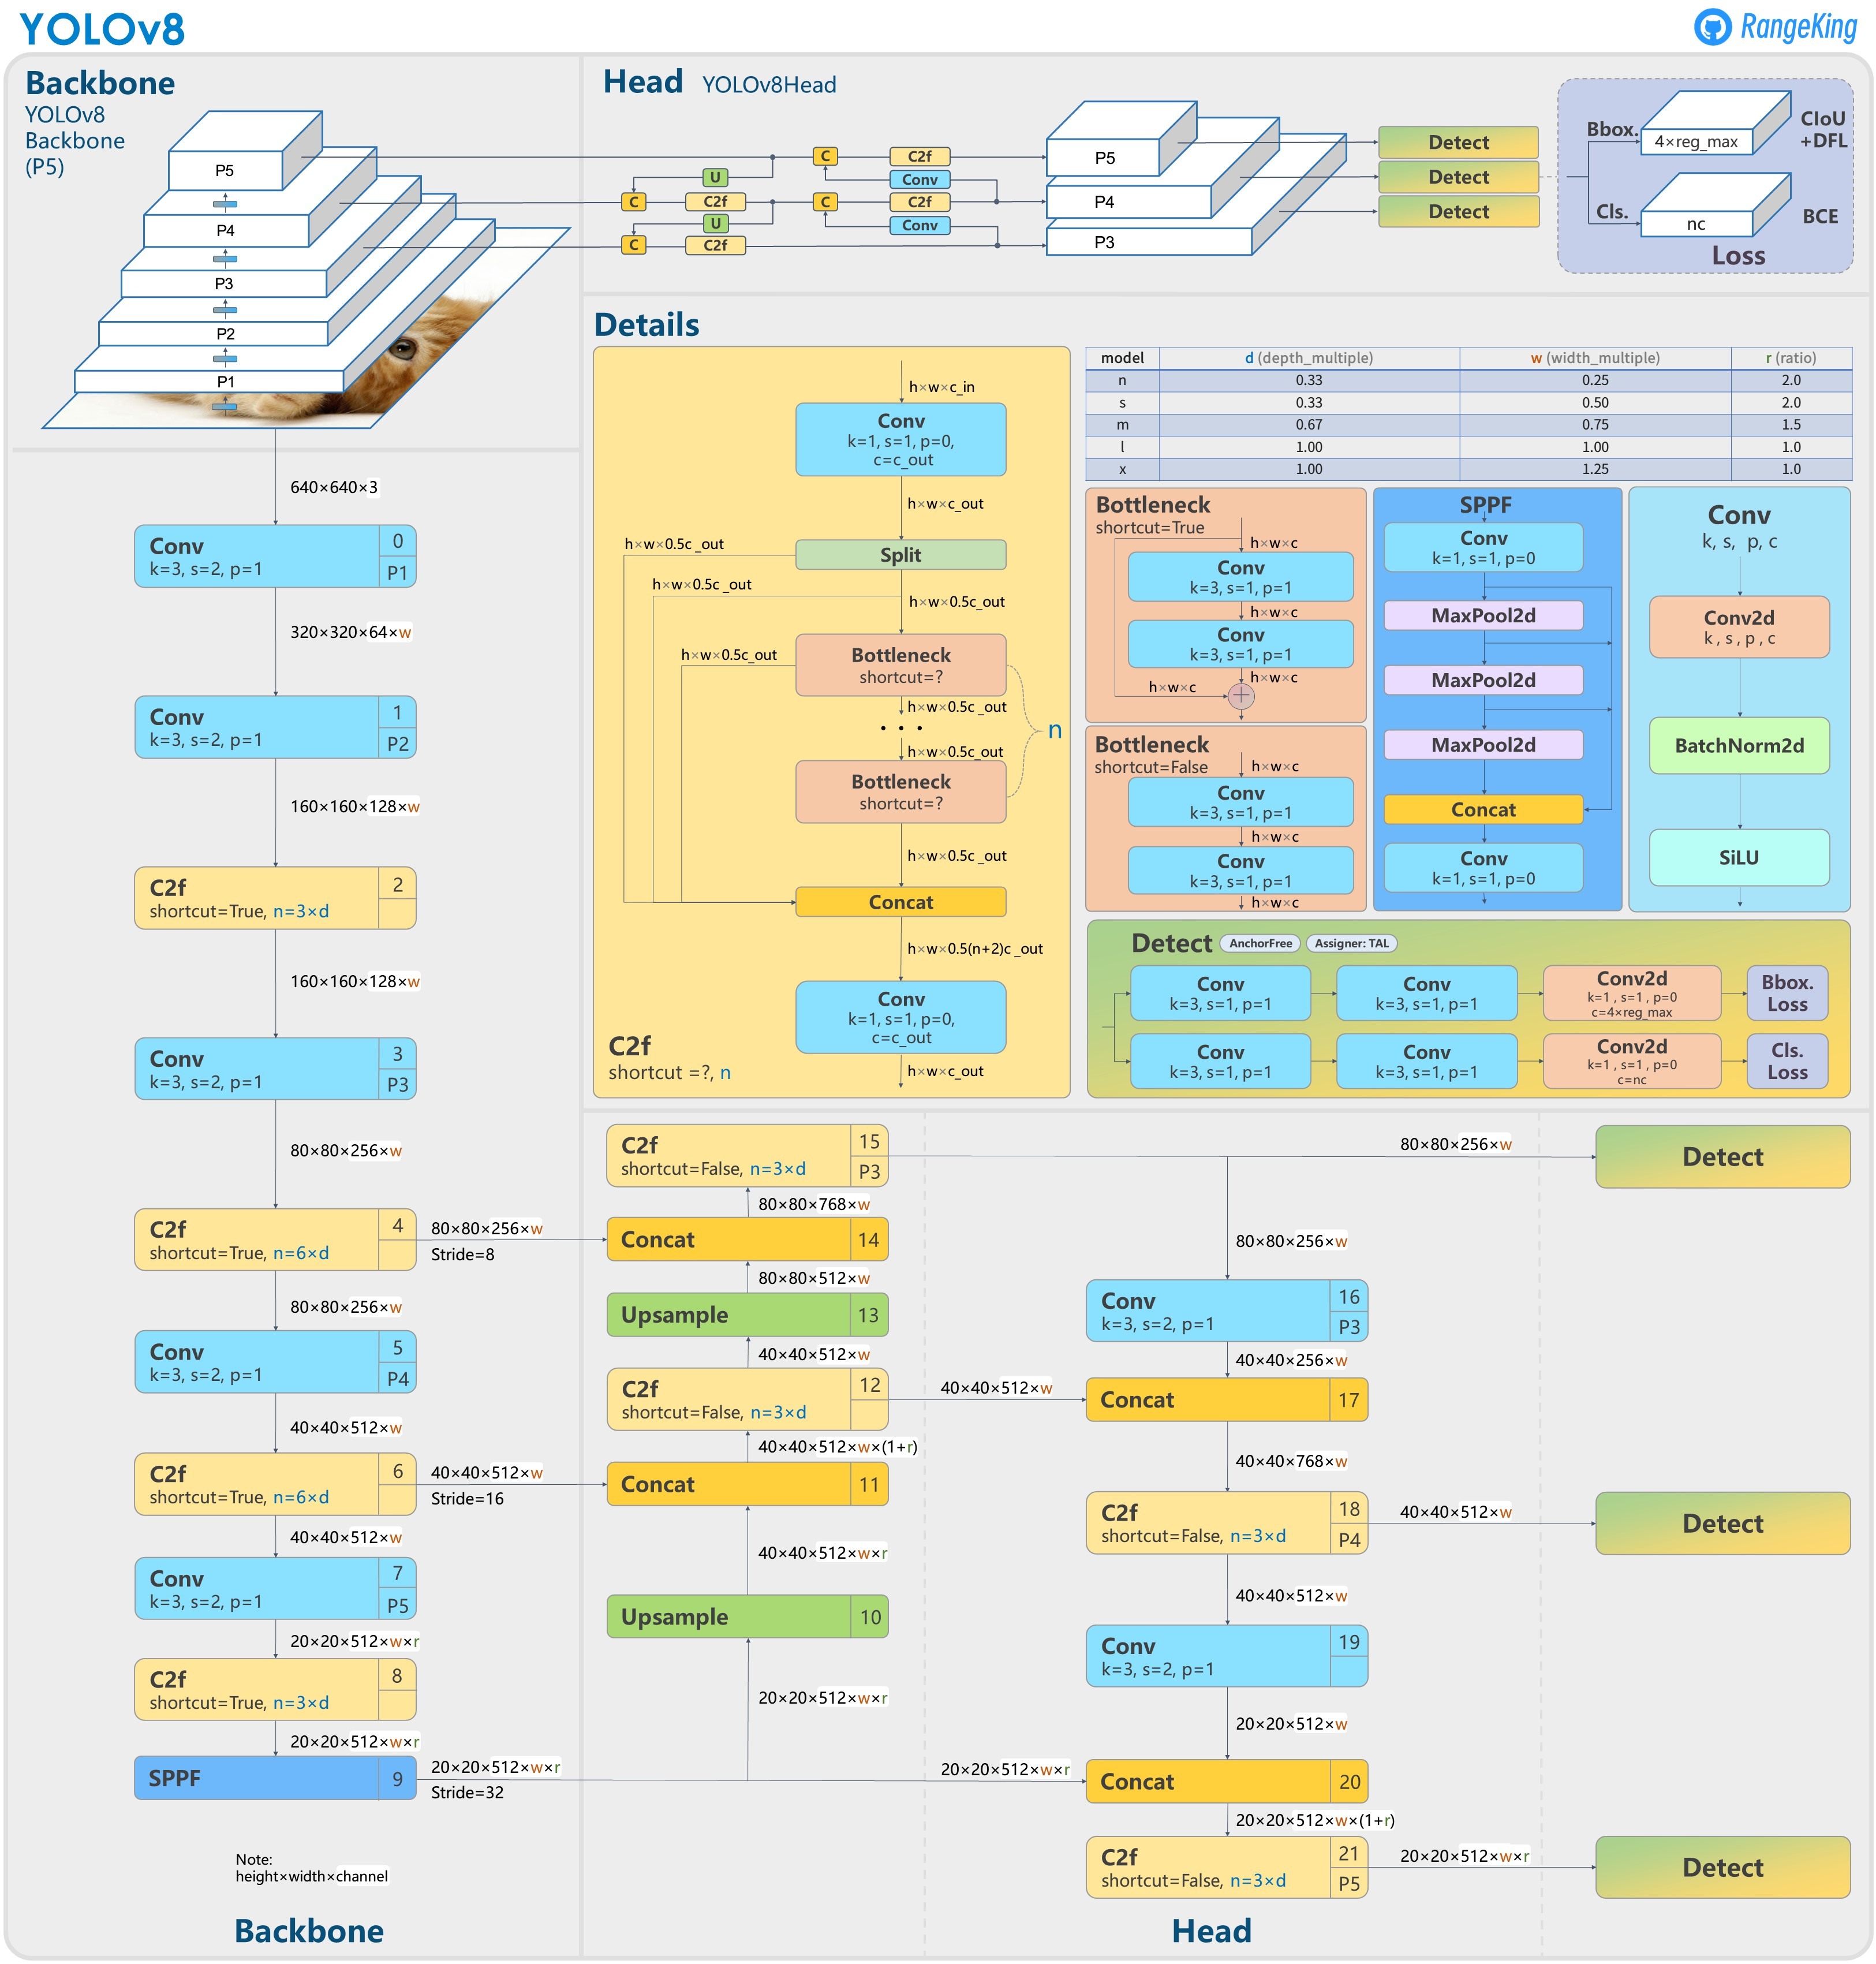
\includegraphics[width=\textwidth]{yolov8_architecture.jpg}
    \caption{Schema dell'architettura di YOLOv8.}
    \label{fig:yolov8_architecture}
\end{figure}

Il modello YOLOv8 incorpora anche una \textit{Neck} e una \textit{Head} ottimizzati per massimizzare la capacità di rilevamento attraverso una migliore aggregazione delle caratteristiche e una maggiore flessibilità nelle predizioni finali. L'uso di meccanismi come le \textit{Depthwise Separable Convolutions} contribuisce a ridurre il numero di operazioni computazionali, mantenendo un'elevata capacità espressiva del modello.
\subsection{Architetture Small e Medium}

Nell'ambito del progetto, si è scelto di utilizzare le varianti \textbf{small} e \textbf{medium} di YOLOv8 per il task di object detection, in quanto queste architetture offrono un buon compromesso tra capacità computazionale e precisione, risultando particolarmente adatte per l'esecuzione su hardware con risorse limitate o in contesti dove è necessaria l'elaborazione in tempo reale.

\begin{itemize}
    \item \textbf{YOLOv8 Small}: Questa versione è progettata per situazioni in cui la velocità è critica e le risorse hardware sono limitate. YOLOv8 Small utilizza un numero ridotto di filtri convoluzionali e strati, il che riduce il numero di parametri complessivi e, di conseguenza, il tempo di inferenza. Nonostante la sua leggerezza, mantiene un'accuratezza adeguata per compiti di object detection su scenari meno complessi o con immagini di bassa risoluzione. È ideale per applicazioni che richiedono una rapida risposta e dove la potenza computazionale è limitata.
    
    \item \textbf{YOLOv8 Medium}: La versione Medium di YOLOv8 rappresenta un'interessante via di mezzo tra precisione e velocità. Questa architettura è più complessa rispetto alla variante Small, con un numero maggiore di strati e parametri, che consente al modello di catturare dettagli più fini e di lavorare meglio su dataset più complessi o con immagini ad alta risoluzione. È particolarmente indicata per scenari dove un compromesso tra velocità e accuratezza è accettabile, garantendo comunque la capacità di rilevare oggetti in tempo reale.
\end{itemize}

\subsection{Vantaggi di YOLOv8 per il Riconoscimento dei Rifiuti Plastici}

La scelta di YOLOv8 per il riconoscimento dei rifiuti plastici nei fiumi è giustificata da diversi fattori:

\begin{itemize}
    \item \textbf{Rilevamento in Tempo Reale}: YOLOv8 è noto per la sua capacità di eseguire object detection in tempo reale, il che è cruciale per applicazioni di monitoraggio continuo nei fiumi. La possibilità di rilevare e classificare i rifiuti plastici in tempo reale consente interventi immediati, riducendo il rischio che i rifiuti possano propagarsi ulteriormente.
    
    \item \textbf{Efficienza Computazionale}: Le versioni Small e Medium di YOLOv8 sono ottimizzate per girare su hardware con risorse limitate, come droni o sistemi embedded. Questo le rende particolarmente adatte per applicazioni sul campo, dove la potenza di calcolo potrebbe essere un vincolo.
    
    \item \textbf{Accuratezza Elevata}: Nonostante la sua velocità, YOLOv8 mantiene un'accuratezza competitiva grazie all'uso di tecniche avanzate come l'addestramento con \textit{label smoothing} e l'adozione di una griglia più fine per la previsione delle bounding box. Questo è essenziale per distinguere efficacemente i rifiuti plastici da altri detriti naturali presenti nei fiumi.
    
    \item \textbf{Robustezza in Ambienti Variabili}: YOLOv8 è progettato per funzionare in diverse condizioni di illuminazione e in presenza di rumore visivo, caratteristico di ambienti naturali come i fiumi. La capacità del modello di generalizzare bene a scenari non ideali è un vantaggio chiave per garantire il successo del sistema di rilevamento.
\end{itemize}

\subsection{Considerazioni Finali}

In conclusione, YOLOv8, nelle sue varianti Small e Medium, rappresenta una scelta ottimale per il progetto di riconoscimento dei rifiuti plastici nei fiumi. La combinazione di efficienza computazionale, accuratezza e capacità di operare in tempo reale rende YOLOv8 particolarmente adatto per implementazioni sul campo. L'architettura del modello, progettata per massimizzare le prestazioni in contesti reali, assicura che il sistema sia in grado di operare efficacemente in ambienti complessi e variabili come quelli fluviali.

\begin{figure}[h!]
    \centering
    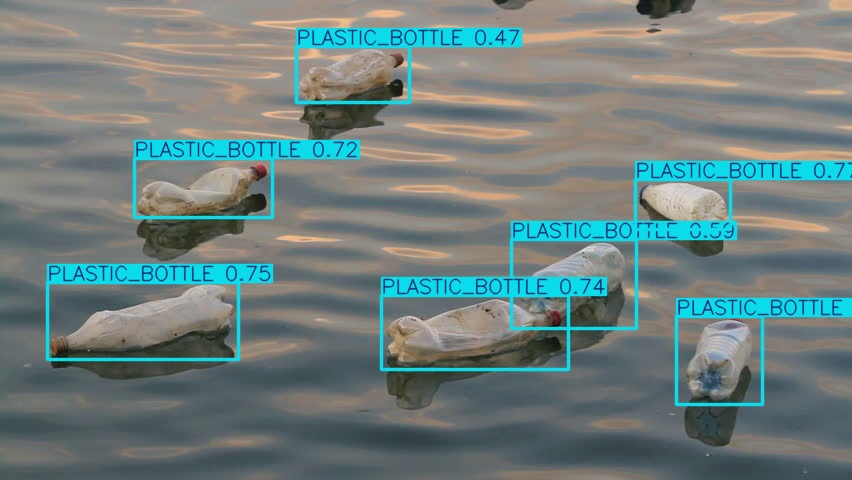
\includegraphics[width=\textwidth]{res_1203_1.jpg} 
    \caption{Esempio di output di YOLOv8 per il rilevamento di rifiuti plastici nei fiumi.}
    \label{fig:yolov8_output}
\end{figure}
